\section{Introduction}
One of the easiest \acrlong{ips} to implement is \acrshort{wlan} (specified by IEEE in their 802.11 specification) \acrshort{ips}. The adoption of such a system comes without extra cost as most of the hardware is already prevalent in large, indoor environments.  The globally adopted operating bandwidth of \acrshort{wlan} is 2.4GHz (IEEE 802.11b, also known as Wi-Fi \cite{Li}), which does not come without its problems as discussed in a later chapter \cite{Techopedia} \cite{ElectronicsNotes}\cite{Cisco}. In this chapter the most commonly used techniques to calculate the position of a \acrlong{mu} and the distance between a \acrlong{tx} and a \acrlong{rx}, being the \acrlong{mu}, are covered. After having covered the specific techniques, this chapter discusses the feasibility of this specific \acrlong{ips} with the complications of the 2.4GHz bandwidth as well as already commercially available systems.
\section{WLAN Characteristics}
\subsection{Signal Properties}
\subsection{Available Channels}
\subsection{Access Points}
\section{Indoor Positioning Topology}
Three topologies exists that can be used for gathering information about the position, as listed below \cite{Henniges2012}:
\begin{enumerate}
\item Network-based topology: position is determined by a central server and different \acrshort{ap}s;
\item Terminal-based: the position is identified by the mobile device;
\item Terminal-assisted: hybrid version of 1. and 2.
\end{enumerate}
\begin{figure}[h!]
\centering
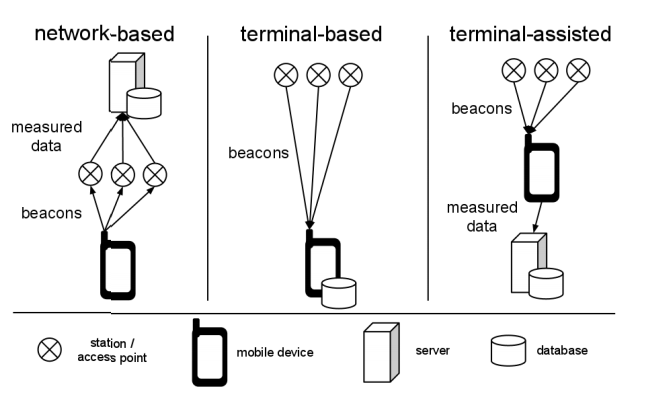
\includegraphics[scale=0.75]{ips_topologies}
\caption{IPS Topologies ~\cite{Henniges2012}}
\label{fig:ips_topologies}
\end{figure}
\subsection{Network-based}
This method only functions when the \acrshort{ap}s are adapted to not only receive network data but also signal data and redirect this to a central server that can handle and compute the data. This requires a change in the software of each \acrlong{ap}.
\subsection{Terminal-Based}
In this specific topology, the device driver of the \acrshort{ap} or terminal broadcasts beacons in its signalling range so a client can determine the best connectivity to a certain \acrshort{ap} and determine which \acrshort{ap} will be used. There are two ways of obtaining this information: active probing and \acrshort{rf} monitoring. The RF monitoring is a form of passive scanning that listens to the periodic broadcasting by the \acrlong{ap}s, this is important to identify a connection in decline (due to significant noise on the signal, also known as \acrfull{snr}) . When using active probing, the driver sends request frames to each known channel to detect any active WLAN connections. Each \acrshort{ap} receiving a request frame will in its turn respond with a response frame. These packets contain the \acrshort{mac} addresses of available devices. Based on this list of available devices and the corresponding signal strength (obtained from services that provide the information via the \acrshort{mac}-layer) an optimal \acrshort{ap} is selected\cite[p.~8]{Retscher}.
\subsection{Terminal-Assisted}
\section{Indoor Positioning Techniques}
The main difficulty in using this technique is determining the position of a device, relative to a Wi-Fi \acrfull{ap}. There are two mainly used technologies to determine the location of a \acrfull{mu}, being: positioning based on \acrshort{rssi} measurements (used in trilateration) and on empirical observations (fingerprinting) \cite{Frank2009}.
\subsection{Proximity or Cell of Origin Technique}
This technique does not result in an absolute or relative position, rather the position of a specific \acrlong{ap} which can then be used to determine a symbolic location. This is a straightforward technique that uses the position of the \acrshort{ap} with the strongest \acrlong{rss} to the \acrlong{mu}. This is an optimal technique to provide symbolic \acrlong{lbs} \cite{Sakpere2017}.
\subsection{Trilateration Technique}
Trilateration, or multilateration, is based on a mathematical approach that incorporate the characteristics of the \acrshort{ap} and its signals, such are: characteristics of the radio signal (wavelength, frequency, noise etc.), \acrfull{mac} address of the \acrlong{ap} and the position of WLAN \acrshort{ap}s, without being limited to taking the signal strength in account. This approach requires three base points to calculate and determine a point in range of these three base points. Applying this method to the current case in which the available base points are the \acrshort{ap}s and the \acrshort{mu}, one has to calculate the distance of the \acrlong{mu} to each of the three \acrshort{ap}s in the vicinity. The main difficulty using this method is the estimation of the distances between both the \acrshort{ap}s and the device. Commonly used methods to determine the distance between both the AP as well as the mobile user include: \, \acrfull{toa} from transmitters or \acrfull{tdoa} \cite[p.~1]{Shchekotov} \cite[p.~60]{Mautz}.
\subsubsection{Geometric Principle}
As stated in the previous paragraph, trilateration requires an equation system containing three distance measurements between \acrshort{ap} and \acrlong{mu}. Using the euclidean distance between two points, this results in the following system or model \cite{CutTheKnot}:
\[ \sqrt{(x-x_1)^2 - (y-y_1)^2} = d_1 \]
\[ \sqrt{(x-x_1)^2 - (y-y_1)^2} = d_2 \]
\[ \sqrt{(x-x_1)^2 - (y-y_1)^2} = d_3 \]
By solving this system of equation, each distance is considered to be the radius of a circle, starting at the \acrshort{ap}. The three circles created by according radius contain an intersection point, the specific location of the user, as visualized in figure 4.1.
\begin{figure}[h!]
\centering
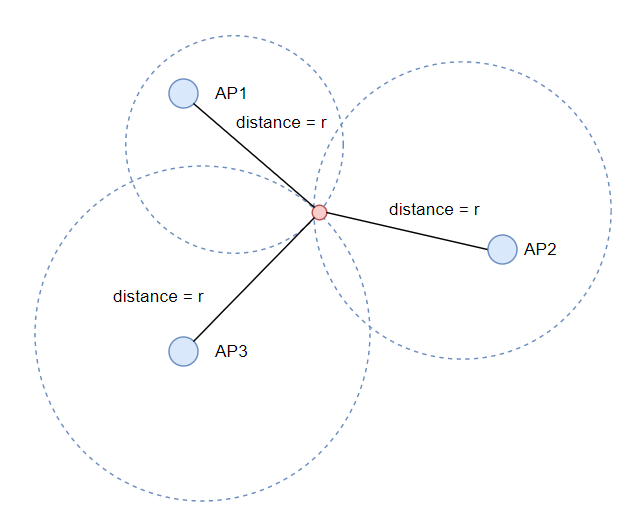
\includegraphics[scale=0.5]{euclidean_distance}
\caption{Euclidean distance resulting in geometric intersection of three circles, determining the position of a point in between these three points.}
\label{fig:euclidean}
\end{figure}
\section{Distance Measurement Techniques}
\subsection{Path Loss Positioning based on RSSI Measurements}
To handle the loss and gain of the radio signal, a free-space path loss model is used, as seen in an experiment in \cite[p.178]{Shchekotov}. Shchekotov's research is funded on the research of Sklar in 1997 that suggests that the average \acrshort{rssi} is distributed lognormally and can therefore be predicted by using a path loss model \cite[p.16]{S2016}. The path-loss model revolves around the calculation of the distance based on the attenuation of the signal \cite{Mautza}.
\begin{figure}[h!]
\centering
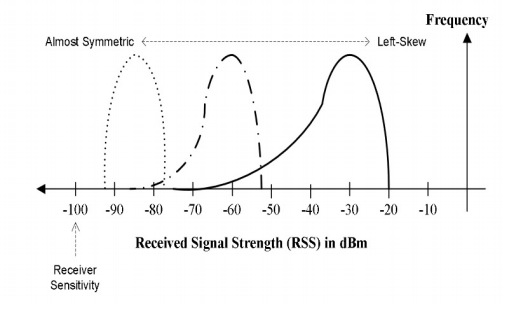
\includegraphics[scale=0.75]{distribution_of_rssi}
\caption{Distribution of ~\acrlong{rssi} ~\cite[p.16]{S2016}}
\label{fig:distribution_rssi}
\end{figure}
\begin{figure}[h!]
\centering
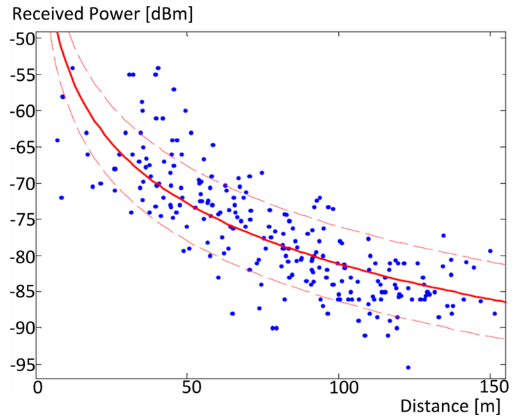
\includegraphics[scale=0.75]{rssi_distance}
\caption{Dependency of ~\acrlong{rssi} and distance ~\cite[p.61]{Mautz}}
\label{fig:rssi_distance}
\end{figure}
The empirical formula, solely based on measurements from the experiment so not a standard analytical model, provided by \cite{S2016} is as follows:
\[
FPSL = 20log10(d) + 20log10(f) - 27.55
\]
Where the \acrlong{tx}-\acrlong{rx} separation distance is annotated by the variable $d$ and the frequence in \acrfull{mhz} by $f$. $FPSL$ indicates the received signal strength path loss in \acrfull{dbm}.
\subparagraph{Conclusion}
Based on the research done in \cite{Shchekotov}, the signal propagation model using a free-space path loss approach does not provide an accurate estimation of the user's current position due to fluctuations in the radio wave channel and decrease of accuracy with an increasing distance \cite[p~61]{Mautz} \cite[p~2]{Loy2018}.
\subsection{RSS Measurement Collection}
This method uses an empirical (observational) model, generated by trial runs using different calibration points with different \acrlong{ap}s. As seen in experiment in \cite{Shchekotov}, this experiments results in a table containing different measurements of different distances and the received signal strength in dBm, from \acrlong{tx} to the \acrlong{rx}. This empirical method results in a usable mathematical formula:
\[
\Delta = \sqrt{\sigma * t)^2 + A^2}
\]
In this equation $\Delta$ annotates the observational error in dBm, $\sigma$ is the standard deviation of the experiment, $t$ is the function of the t-distribution and $A$ is the observational error of the \acrfull{rx} ~\cite[p.178]{Shchekotov}.
\begin{figure}[h!]
\centering
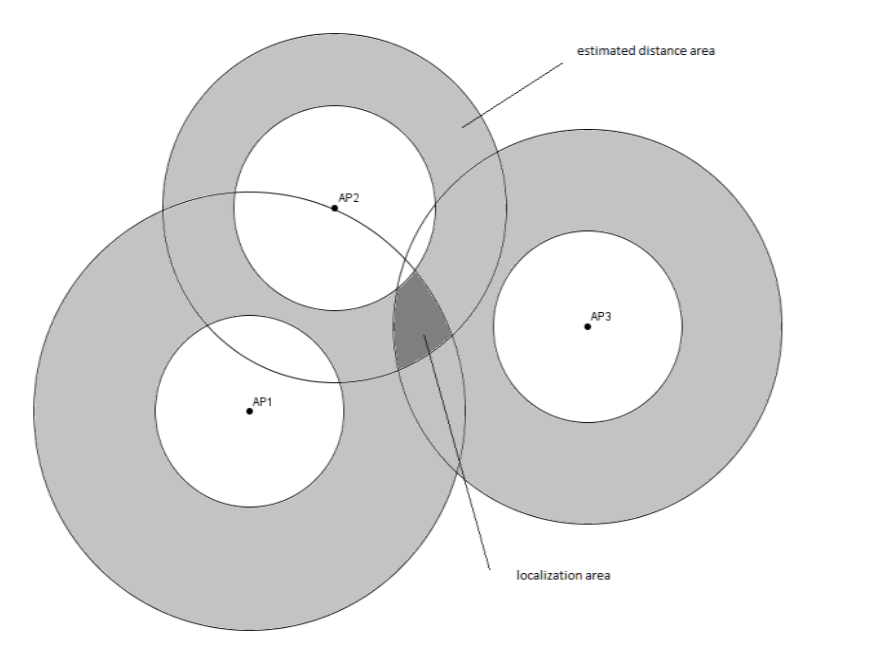
\includegraphics[scale=0.5]{estimated_distance_segments}
\caption{Estimated distance segments ~\cite[p.179]{Shchekotov}}
\label{fig:estimated_distance_segments}
\end{figure}
\subparagraph{Conclusion}
As seen in the trials performed in the research of \cite{Shchekotov}, this approach can be perceived as a special case of fingerprinting due to the creation of a \acrshort{rss} to \acrshort{ap} table. This method results in a more accurate estimation of the user's location by taking the error and deviation into account. However, this research was not based on extensive measurements and it is uncertain this approach will yield an optimal accuracy and precision.
\subsubsection{Time of Arrival}
\subsubsection{Time Difference of Arrival}
\subsubsection{Angle of Arrival}
To enable the use of the \acrshort{aoa} method, the network needs to be equipped with additional directional antennae that are able to calculate the distance. Based on this requirement alone, which comes at a high cost, this approach is not feasible for production environments .
\subsubsection{Round Trip Time}
\subsection{Fingerprinting Technique}
A computationally effective method of determining a user's location is the fingerprinting technique. This technique consists of two phases: offline acquisition of \acrshort{rssi} values at particular locations and an online phase with the actual implementation of periodically sent signals from a \acrshort{mu} \cite[p.~9]{Retscher}. This method bases itself only on the strength of the signal compared to trilateration that incorporates multiple methods to calculate the distance.
\begin{figure}[h!]
\centering
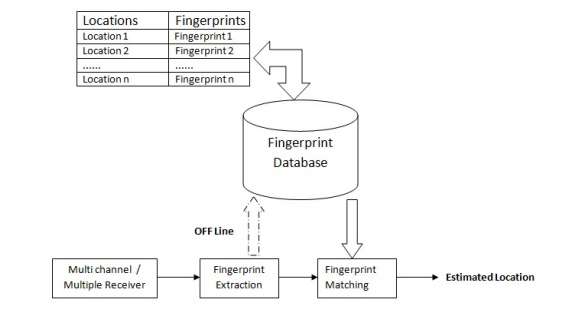
\includegraphics[scale=1]{fingerprint_chart}
\caption{Fingerprinting Stages ~\cite[p.11]{S2016}}
\label{fig:fingerprint_chart}
\end{figure}
\begin{figure}[h!]
\centering
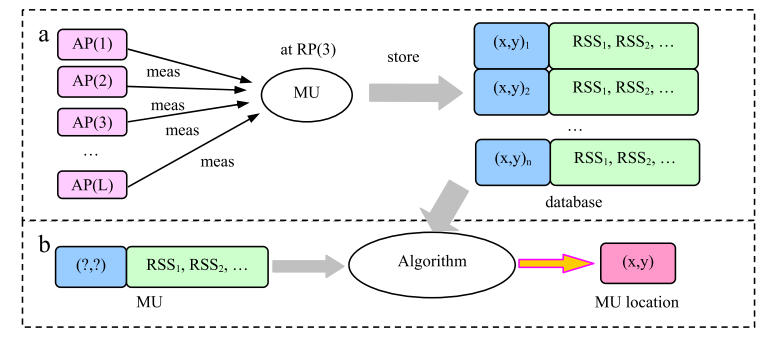
\includegraphics[scale=0.75]{fingerprinting_stages}
\caption{Fingerprinting Stages ~\cite[p.2]{Li}}
\label{fig:fingerprint_stages}
\end{figure}
\subsubsection{Offline Acquisition}
The offline stage of fingerprinting consists of defining and measuring calibration points, which is a major drawback as this is a time-consuming task. The result of the empirical measurements of different points is a radio map with signal strengths in relation to the specific points. The \acrshort{rssi} is measured a few times on each calibration points and afterwards stored inside a database. Each entry in the database is a fingerprint, f, with a corresponding ground-truth (\acrshort{rssi}), symbolized as a vector in a three dimensional vector space.
\subsubsection{Online Phase}
In the online phase, the fingerprints stored in the database are used to determine and estimate the current position of a \acrshort{mu}. The estimation of the distance is in most cases calculated using the Euclidean distance method as shown in \cite{fig:euclidean}. The most straightforward method is to determine the minimum distance between the observation (current position) and the \acrshort{ap}s in the vicinity. Another method is a probabilistic method that calculates the probability that the current \acrlong{rssi} measurements have the same position as a fingerprint corresponding in the fingerprint database \cite{Mautz}. This approach is based on the correlation values of the current observation and the fingerprints available in the database. This requires additional computing power but results in an increased accuracy.
\subsubsection{Improving Performance}
Contributing factors to increasing the performance, mainly accuracy and precision, are: number of \acrshort{ap}s per $m^2$, the amount of calibration points measurement in the offline phase, the density of those points and the fluctuations in  \acrshort{rssi} values.
\subparagraph{Conclusion}
This method requires a lot of time to set up the radiomap in the offline phase, but results in a satisfactory accuracy, generally several meters, and precision. This is the preferred method of providing indoor location using a \acrshort{wlan}-based technology as it does not require additional equipment to be installed or configured. However, this technique is complex, hard to initially set up and does not scale well with an increase in users due to the increasing fluctuations in the radio signal that arise because of environmental factors.
\section{Feasibility}
\subsection{Security and Privacy}
\subsection{Cost}
\subsection{Performance}
\subsection{Environmental Effects on Radio Frequency and Fault Tolerance}
Radio frequency signals are subjected to interference from other signals. This included reflection, diffraction and scattering. These interferences on a radio frequency signal can result in a loss of accuracy and precision in an \acrlong{ips} and are therefore implications of this specific indoor positioning technology \cite{S2016}. 
\subsubsection{Indoor Environment}
Based on a study performed in \cite{Wang2003}, where the signal strength of a 2.4GHz radio wave was tested over a period of 24 hours, the signal strength contains some interferences but overall results in a mean signal strength of 47.17dBm. In \cite{fig:wang_test} the samples of the experiment are plotted in function of the time.
\begin{figure}[h!]
\centering
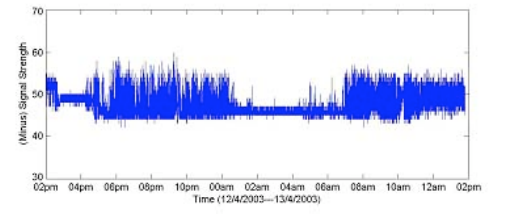
\includegraphics[scale=1]{wang_test}
\caption{24 hour static signal strength measurements ~\cite{Wang2003}}
\label{fig:wang_test}
\end{figure}
\subparagraph{Conclusion of experiment conducted in ~\cite{Wang2003}}
The experiment concludes that the radio signal of a WLAN infrastructure, operating on a 2.4GHz frequency, is stable and consistent, thus this signal can be used in calculations for positioning algorithms. However, the developer of such an algorithm needs to take the standard deviation into account as this differs throughout the use of different indoor environments, even on the level of floors, meaning that the signal strength on the first floor can differ on the third, based on environmental changes (e.g. moving persons, microwaves, other interfering electronic devices).
\subsubsection{SNR in WLAN}
The signal to noise ratio is the difference between the signal strength and the interfering signals. This is a facotr to take into account when deploying any \acrshort{wlan} \acrlong{ips}. A satisfactory \acrlong{snr} should lie above 20 to 25 \cite{Hallock2015}.
\subsubsection{Signal Attenuation}
Signal attenuation, or signal loss, represents the loss of signal strength in \acrfull{db} of radio signals travelling through certain objects. The most common objects and their derived signal attenuation are represented below:
\begin{table}[]
\centering
\begin{tabular}{|l|l|}
\hline
\textbf{Object}             & \textbf{Signal Attenuation} \\ \hline
Plasterboard wall           & 3 dB                        \\ \hline
Glass wall with metal frame & 6 dB                        \\ \hline
Cinder block wall           & 4 dB                        \\ \hline
Office window               & 3 dB                        \\ \hline
Metal door                  & 6 dB                        \\ \hline
\end{tabular}
\caption{Objects with corresponding signal attenuation ~\cite[p.99]{Hallock2015}}
\end{table}
\subsubsection{Human Body}
The human body also has an effect on signals that are transmitted through the human body. As seen in the experiment by \cite{S2016} the difference of the standard deviation is 2.32dBm. The research conducted in \cite{Mautz} even reports a measurement error of nearly 15dBm.
This is why the fingerprinting technique is the favourable method to estimate the current position of a \acrlong{mu}, the fingerprinting provides a fault-tolerant method due to the multiple calibration measurements conducted in the offline phase, where the calibration should include signals passing through the human body.
\subsection{Complexity}
\subsection{Application Use}
\subsection{Commercial Availability}
\subsubsection{RADAR}
\subsubsection{COMPASS}
\subsubsection{Ekahau}
\section{Conclusion}
